\documentclass[compress]{beamer}
\usepackage[utf8]{inputenc}
\usepackage[T1]{fontenc}
\usetheme{Singapore}
\usecolortheme{default}
\usepackage{graphicx}

\begin{document}
\title{Verschlüsselung mit GPG}  
\author{Sokü \& friends}
\date{} 

\frame{\titlepage} 

\frame{
  \frametitle{Struktur}
  \tableofcontents
} 

\section{Motivation}
\label{sec:motivation}

\begin{frame}
  \frametitle{Warum das alles eigentlich?}

  \begin{itemize}[<+(1)->]
  \item Emails sind unsicher
  \item Nur wer ein bisschen die Technik versteht, kann sich bewusst
    verhalten
  \end{itemize}
\end{frame}

\section{Theorie}
\label{sec:theorie}
\frame{ \frametitle{\insertsection}
  Etwas trockener Hintergrund ist leider notwendig.  Aber wir
  machen es ganz kurz! }

\subsection{Symmetrische und Asymmetrische Verschlüsselung}
\begin{frame}
  \frametitle{\insertsubsection}
  \begin{overprint}
    \onslide<1-4>
    \begin{description}
    \item[Früher] symmetrische Verschlüsselung: \alert{ein} Schlüssel
      zum Verschlüsseln und wieder Entschlüsseln\only<4>{, Schlüssel muss
      sicher von der Senderin zum Empfänger gebracht werden (alte
      Agentenfilme: Aktenkoffer mit Selbstzerstörung, das ist doch
      aufwändig)}
    \end{description}
    \onslide<5-7>
    \begin{description}
    \item[New \& hot] Asymmetrische Verschlüsselung mit zwei
      Schlüsseln: \alert{öffentlicher} nur zum Verschlüsseln (darf
      auch den Bösen bekannt sein) und \alert{privater} zum
      Entschlüsseln (geheim, muss aber nicht mehr quer durch die Stadt
      getragen werden)
    \end{description}
    \onslide<8>
    \begin{description}
    \item[Wie geht das?] Mathe!  Zahlen multiplizieren geht leicht,
      Zahlen wieder aufteilen nicht.
    \end{description}
  \end{overprint}
  \vspace{1em}
  \begin{overlayarea}{\columnwidth}{8em}
    \includegraphics<2>[width=\columnwidth]{bilder/symmetric_schluessel.png}
    \includegraphics<3>[width=\columnwidth]{bilder/symmetric_text.png}
    \only<4>{
      \begin{center}
        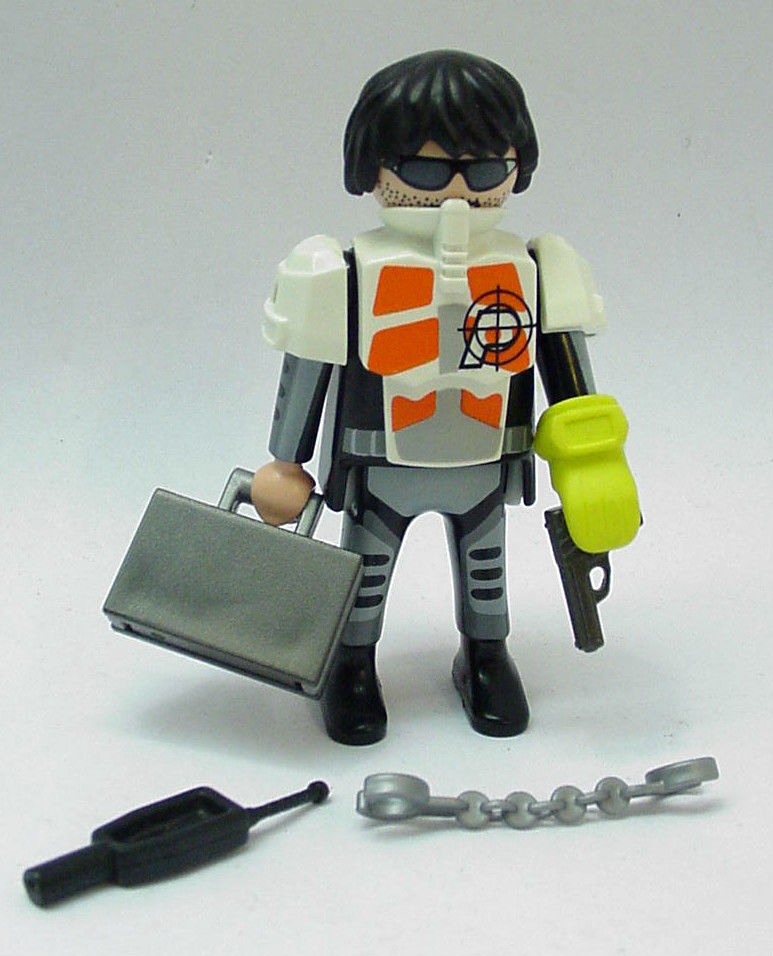
\includegraphics[height=9em]{bilder/agent_koffer.jpg}
      \end{center}
    }
    \includegraphics<6>[width=\columnwidth]{bilder/public_key_verfahren_schluessel.png}
    \includegraphics<7>[width=\columnwidth]{bilder/public_key_verfahren_text.png}
  \end{overlayarea}

\end{frame}

\subsection{Primzahlen rechnen}
\begin{frame}
  \frametitle{\insertsubsection}
  \begin{description}
  \item[Taschenrechner dabei?]
    \begin{itemize}
    \item 7 x 11 = ?
    \item 65 = ? x ? (5 x 13)
    \item 11251 x 2953 = 33224203
    \item 12883649 = ? (2957 x 4357) kann wohl niemand in unter einem
      Tag ausrechnen, auch mit Taschenrechner
    \end{itemize}
  \item[Verschlüsselung?] Das Produkt aus den zwei Primzahlen ist in
    etwa der öffentliche Schlüssel (auch die Geheimdienste können die
    Zahl nicht wieder aufspalten), die zwei kleinen Zahlen sind der
    private Schlüssel und müssen geheim bleiben.
  \end{description}
\end{frame}

\section{Theoretische Praxis}
\label{sec-1-1-4}

Schlüsselerstellung (Zufall), Schlüsselaustausch, Schlüsselserver,
Fingerprints, Signaturen (Keysigning-Parties), Widerrufszertifikat,
Email (Betreff, Header, Anhänge)

Abgrenzen zu:
\begin{itemize}
\item Festplattenverschlüsselung
\item Apps auf Handys/Smartphones, Chat
\item Anonymität
\end{itemize}
\section{Die Praxis in der Theorie}
\label{sec-1-1-5}

GPG4Win, Enigmail, sonstige Programme

Screenshots: Installation, Schlüsselgenerierung
(Widerrufszertifikat!), Einrichtung Enigmail, Schlüssel hochladen,
Schlüssel runterladen, Mail versenden, Mail empfangen
\section{Praktische Praxis}
\label{sec-1-1-6}

\begin{itemize}
\item Runterladen/Verteilen
\item Installieren
\item \ldots{} (wie oben)
\end{itemize}

Vielleicht zuerst eine Mail an sich selber schreiben?
\section{Weiterführendes}
\label{sec-1-1-7}

\begin{itemize}
\item Skript?
\item Feedbackrunde
\item Weitere Wünsche?
\end{itemize}

\section{Section no.1} 
\frame{\frametitle{Title} 
Each frame should have a title.
}
\subsection{Subsection no.1.1  }
\frame{ 
Without title somethink is missing. 
}


\section{Section no. 2} 
\subsection{Lists I}
\frame{\frametitle{unnumbered lists}
\begin{itemize}
\item Introduction to  \LaTeX  
\item Course 2 
\item Termpapers and presentations with \LaTeX 
\item Beamer class
\end{itemize} 
}

\frame{\frametitle{lists with pause}
\begin{itemize}
\item Introduction to  \LaTeX \pause 
\item Course 2 \pause 
\item Termpapers and presentations with \LaTeX \pause 
\item Beamer class
\end{itemize} 
}

\subsection{Lists II}
\frame{\frametitle{numbered lists}
\begin{enumerate}
\item Introduction to  \LaTeX  
\item Course 2 
\item Termpapers and presentations with \LaTeX 
\item Beamer class
\end{enumerate}
}
\frame{\frametitle{numbered lists with pause}
\begin{enumerate}
\item Introduction to  \LaTeX \pause 
\item Course 2 \pause 
\item Termpapers and presentations with \LaTeX \pause 
\item Beamer class
\end{enumerate}
}

\section{Section no.3} 
\subsection{Tables}
\frame{\frametitle{Tables}
\begin{tabular}{|c|c|c|}
\hline
\textbf{Date} & \textbf{Instructor} & \textbf{Title} \\
\hline
WS 04/05 & Sascha Frank & First steps with  \LaTeX  \\
\hline
SS 05 & Sascha Frank & \LaTeX \ Course serial \\
\hline
\end{tabular}}


\frame{\frametitle{Tables with pause}
\begin{tabular}{c c c}
A & B & C \\ 
\pause 
1 & 2 & 3 \\  
\pause 
A & B & C \\ 
\end{tabular} }


\section{Section no. 4}
\subsection{blocs}
\frame{\frametitle{blocs}

\begin{block}{title of the bloc}
bloc text
\end{block}

\begin{exampleblock}{title of the bloc}
bloc text
\end{exampleblock}


\begin{alertblock}{title of the bloc}
bloc text
\end{alertblock}
}

\section{Section no. 5}
\subsection{split screen}

\frame{\frametitle{splitting screen}
\begin{columns}
\begin{column}{5cm}
\begin{itemize}
\item Beamer 
\item Beamer Class 
\item Beamer Class Latex 
\end{itemize}
\end{column}
\begin{column}{5cm}
\begin{tabular}{|c|c|}
\hline
\textbf{Instructor} & \textbf{Title} \\
\hline
Sascha Frank &  \LaTeX \ Course 1 \\
\hline
Sascha Frank &  Course serial  \\
\hline
\end{tabular}
\end{column}
\end{columns}
}

\subsection{Pictures} 
\frame{\frametitle{pictures in latex beamer class}
%\begin{figure}
%\includegraphics[scale=0.5]{PIC1} 
%\caption{show an example picture}
%\end{figure}
}

\subsection{joining picture and lists} 

\frame{
  \frametitle{pictures and lists in beamer class}
  \begin{columns}
    \begin{column}{5cm}
      \begin{itemize}
      \item<1-> subject 1
      \item<3-> subject 2
      \item<5-> subject 3
      \end{itemize}
      \vspace{3cm} 
    \end{column}
    \begin{column}{5cm}
      \begin{overprint}
% \includegraphics<2>{PIC1}
% \includegraphics<4>{PIC2}
% \includegraphics<6>{PIC3}
      \end{overprint}
    \end{column}
  \end{columns}
}

\end{document}
